


\documentclass[t]{beamer}
\usepackage{lmodern, multirow, bm, threeparttable, booktabs} % to use fonts in different sizes
\usepackage[export]{adjustbox}
 \usetheme{BaylorTheme}

\newcommand{\matr}[1]{\mathbf{#1}}
\addtobeamertemplate{frametitle}{\let\insertframetitle\insertsectionhead}{}
\addtobeamertemplate{framesubtitle}{
\ifx\insertsubsubsectionhead\@empty{\let\insertframesubtitle\insertsubsectionhead}
  \else {{\let\insertframesubtitle\insertsubsectionhead : \insertsubsubsectionhead}{}}
\fi}

 % \usecolortheme{beaver}
 \usecolortheme{bears}

%\setbeamerfont{caption}{size=\footnotesize}

\title[Baylor Theme]{Extensions of Beta Regression for Modeling a Covariate-Specific ROC Curve}
\author[Frank]{Katie Frank} %
\date{Spring 2020}


\begin{document}


\begin{frame}
  \titlepage
  \begin{center}
    
\includegraphics[scale=0.6]{BU_BrandMark_Horz_Green}
  \end{center}
\end{frame}

%%%%% MOTIVATION
\section{Motivation}

\begin{frame}
\frametitle{Motivation}
I will add Motivation last.
\end{frame}

%%%%% OUTLINE
\section{Outline}

\begin{frame}[allowframebreaks]
\frametitle{Table of Contents}
\begin{itemize}
    \item Background
    \begin{itemize}
        \item Evaluating Diagnostic Tests
        \item ROC and AUC
        \item Placement Values
    \end{itemize}
    \item ROC Regression Methodologies
    \begin{itemize}
        \item Parametric Distribution-Free
        \item Beta 
        \item Variable Dispersion Beta
    \end{itemize}
    \item Applications
    \begin{itemize}
        \item Binormal Simulation
        \item Indian Liver Patient Dataset
    \end{itemize}
    \item Conclusion and Future Work
\end{itemize}

\end{frame}


%%%%% PERFORMANCE OF DIAGNOSTIC TESTS
\section{Performance of Diagnostic Tests}

\begin{frame}
\frametitle{Introduction}
\begin{itemize}
	\item The performance of a diagnostic test can be summarized with the true positive rate (TPR) or sensitivity and the false positive rate (FPR) or ($1 -$ specificity).
	\item The TPR is the proportion of diseased subjects ($D = 1$) correctly identified as positive by the test.
	\item The FPR is the proportion of non-diseased subjects ($D = 0$) incorrectly identified as positive by the test.
	\item For a continuous test result $Y$ at threshold $y$, the TPR and FPR are
\end{itemize}
\begin{align*}
	\text{TPR}(y) &= P(Y \geq y| D = 1) \\
	\text{FPR}(y) &= P(Y \geq y| D = 0) \\
\end{align*}
\end{frame}

%%%%% THE ROC CURVE
\section{The ROC Curve}

\begin{frame}
\frametitle{BLAHH}
\begin{itemize}
\item The receiver operating characteristic (ROC) curve is a plot of the TPRs vs. FPRs for all possible cutpoints based on $Y$:
\end{itemize}
$$\text{ROC}(\cdot) = \left\{(\text{FPR}(y), \text{TPR}(y)), \, y \in (-\infty, \infty) \right\}.$$
\vspace{-.2in}
\begin{itemize}
    \item The ROC curve can be represented in terms of survival functions.
    \begin{itemize}
        \item Let $Y_D$ and $Y_{\bar{D}}$ denote the random variables of test results from diseased ($D$) and non-diseased populations ($\bar{D}$),  respectively.
        \item Denote the survival functions of $Y_D$ and $Y_{\bar{D}}$ by $S_D(\cdot)$ and $S_{\bar{D}}(\cdot)$.
    \end{itemize}
\end{itemize}
$$\text{ROC}(t) = S_D(S_{\bar{D}}^{-1}(t)), \quad t \in (0, 1),$$
\vspace{-.2in}
\begin{itemize}
    \item[]
\begin{itemize}
    \item[] where $t$ is the FPR.
\end{itemize}
\end{itemize}
\end{frame}

%%%%% AUC
\section{AUC}

\begin{frame}
\frametitle{AUC}
\begin{itemize}
\item The area under the curve (AUC) is a popular index used to summarize the ROC curve.
\end{itemize}
$$\text{AUC} = \int_0^1\text{ROC}(t)dt.$$
\begin{itemize}
\item It is the probability that a randomly chosen diseased subject has a test result value higher than a randomly chosen non-diseased subject (Hanley and McNeil 1982):
\end{itemize}
$$P(Y_D > Y_{\bar{D}}).$$
\vspace{-.2in}
\begin{itemize}
\item A perfect test has $\text{AUC} = 1.0$.
\item An uninformative test is one such that $\text{ROC}(t) = t$, which has $\text{AUC} = 0.5$.
\end{itemize}
\end{frame}


%%%%% ILLUSTRATING THE AUC
\section{Illustrating the AUC}

\begin{frame}
\frametitle{Illustrating the AUC}
\begin{center}
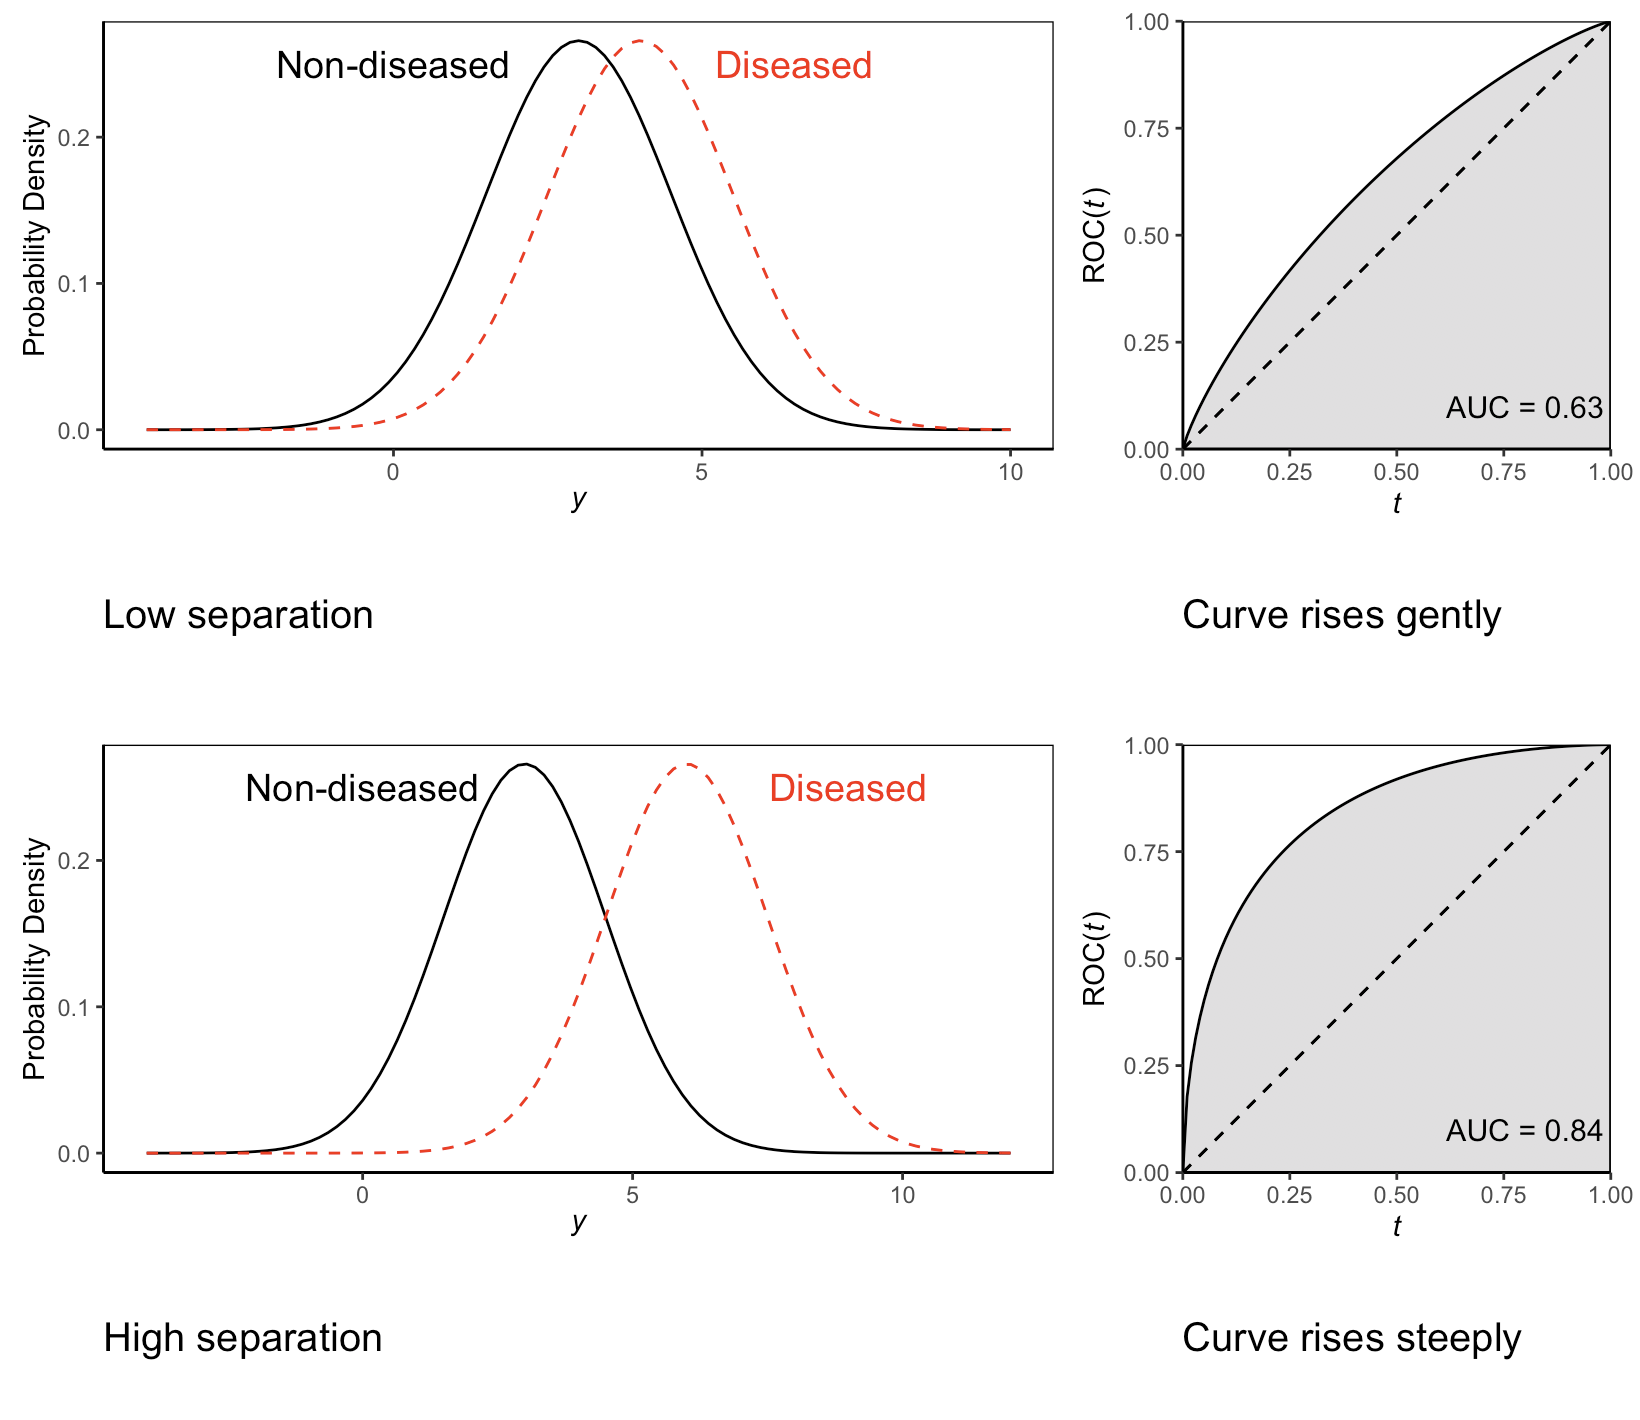
\includegraphics[width=3.5in]{plots}
\end{center}
\end{frame}

%%%%% PLACEMENT VALUES
\section{Placement Values}

\begin{frame}
\frametitle{BLAHH}
\begin{itemize}
\item The placement value of $Y$, $\text{PV}$, is the proportion of the non-diseased population with test values greater than $Y$:
\end{itemize}
$$\text{PV} = S_{\bar{D}}(Y),$$
\begin{itemize}
\vspace{-.2in}
\item[] where $S_{\bar{D}}(\cdot)$ denotes the non-diseased survival function.
\item The ROC curve is the cumulative distribution function (cdf), $\Psi_{\text{PV}}(\cdot)$, for the diseased placement values (Pepe and Cai 2004).
\end{itemize}
\begin{align*}
\Psi_{\text{PV}}(t) &=
P(\text{PV}_D \leq t)\\ &= P(S_{\bar{D}}(Y_D) \leq t) \\
	&= P(S_{\bar{D}}^{-1}(t) < Y_D) \\
	&= S_D(S_{\bar{D}}^{-1}(t)) \\
	&= \text{ROC}(t), \quad t \in (0, 1).
\end{align*}
\vspace{-.2in}
\begin{itemize}
\item[]
\begin{itemize}
\item $\text{PV}_{\bar{D}} = S_{\bar{D}}(Y_{\bar{D}})$ is $\text{Uniform}(0, 1)$.
%\item The distribution of placement values in the diseased population, $\text{PV}_D = S_{\bar{D}}(Y_D)$, quantifies the separation between the two populations.
\end{itemize}
\end{itemize}
\end{frame}

%%%%% ILLUSTRATING PLACEMENT VALUES
\section{Illustrating Placement Values}

\begin{frame}
\frametitle{BLAHH}
\begin{itemize}
\item For highly separated populations, most of the diseased test results $Y_{D_i}, \, i = 1, \dots, n_D$, are greater than the non-diseased test results $Y_{\bar{D}_j}, \, j = 1, \dots, n_{\bar{D}},$ so that the diseased placement values will tend to be small.
\end{itemize}
\begin{center}
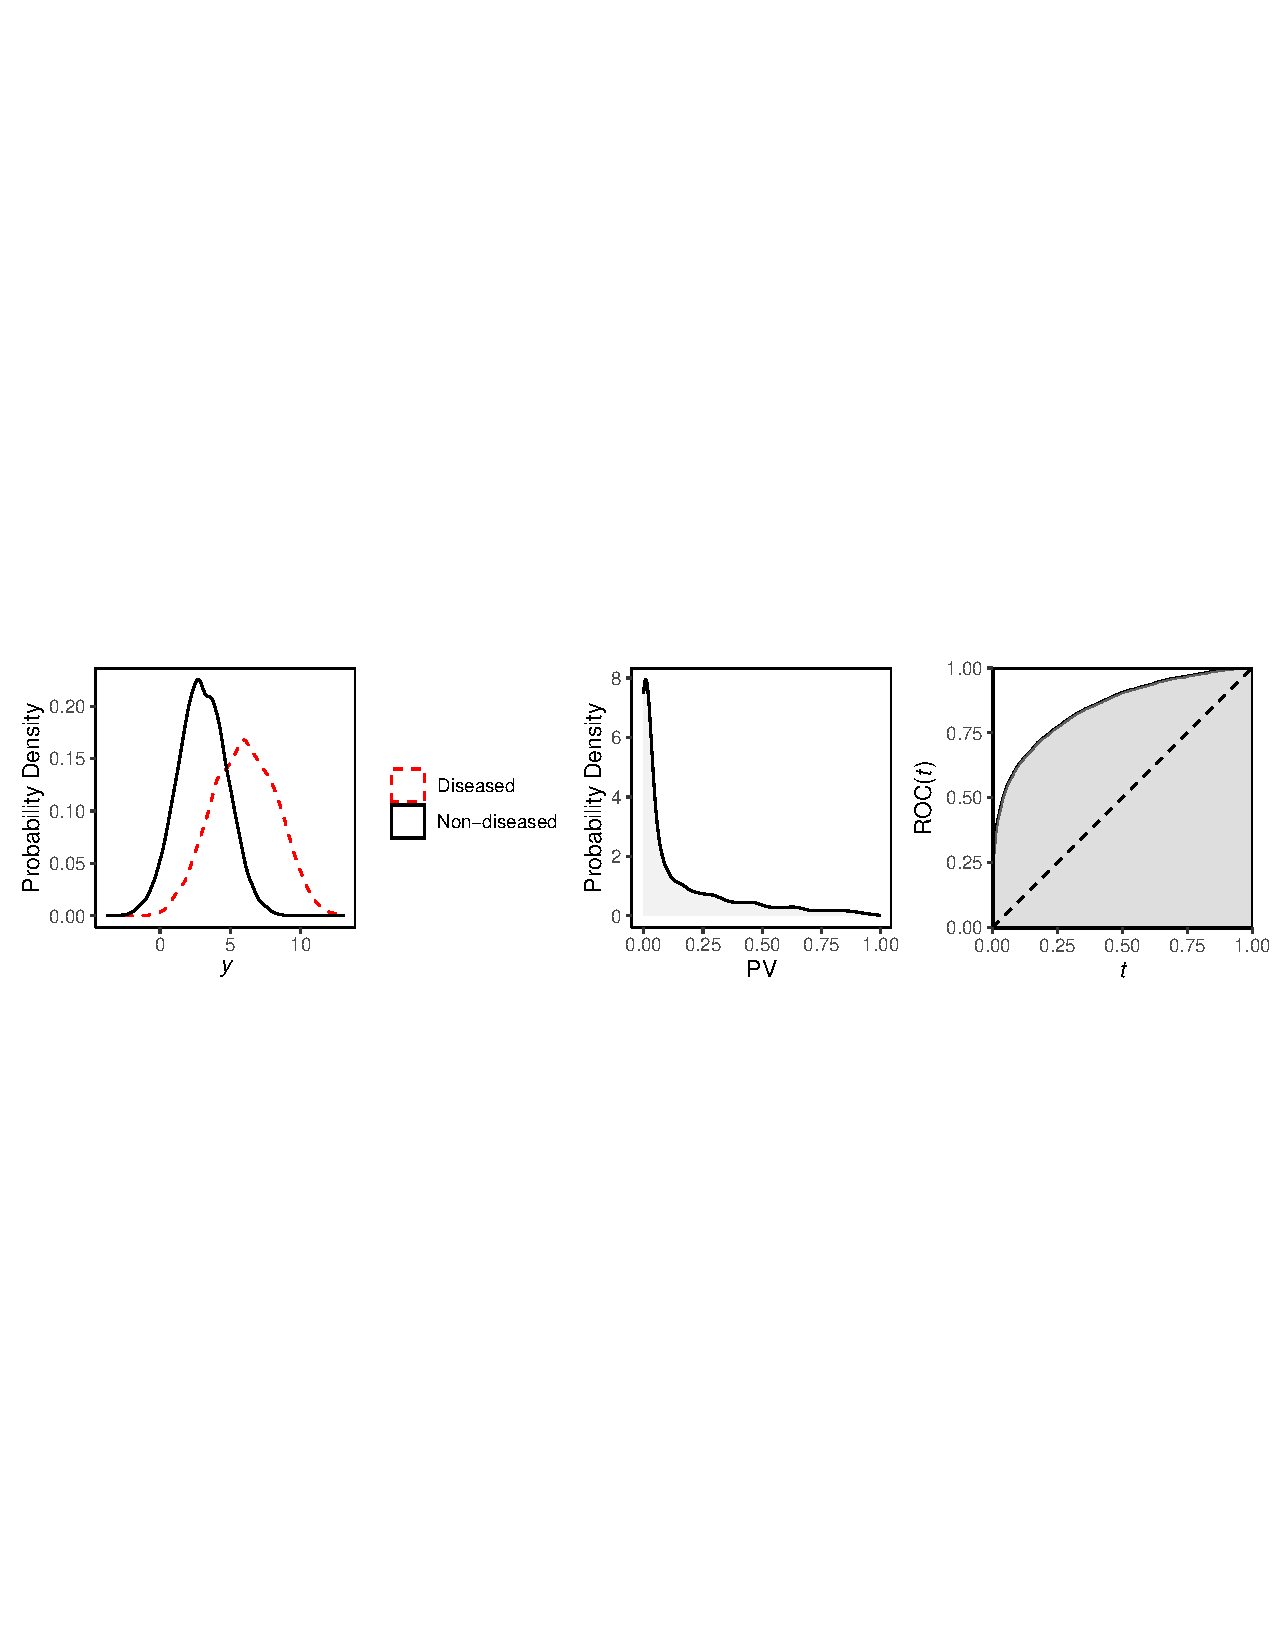
\includegraphics[scale=0.55]{PVs_ROC_high}
\end{center}
\end{frame}

%%%%% ILLUSTRATING PLACEMENT VALUES
\section{Illustrating Placement Values}
\begin{frame}
\frametitle{BLAHH}
\begin{itemize}
\item For overlapping populations, larger diseased placement values will occur more often.
\end{itemize}
\begin{center}
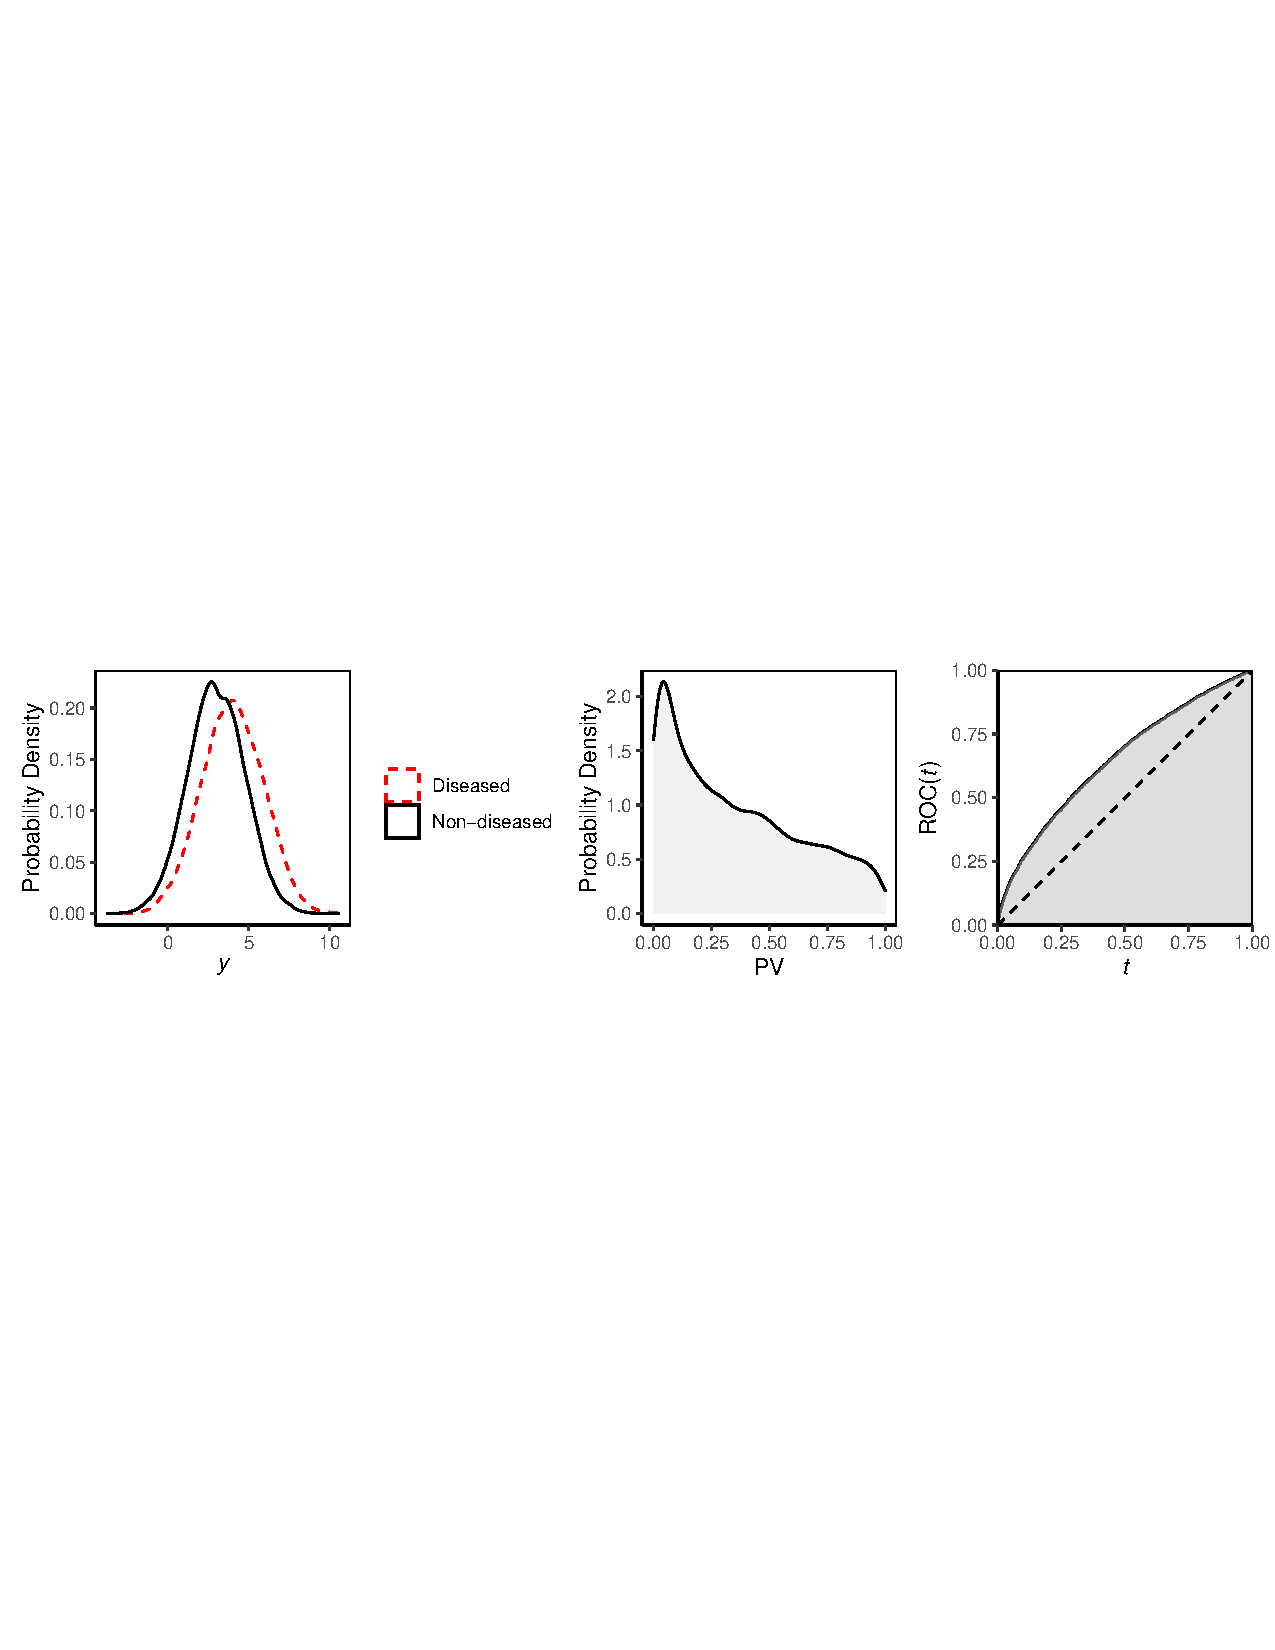
\includegraphics[scale=0.55]{PVs_ROC_low}
\end{center}
\end{frame}

%%%%% PLACEMENT VALUES AND THE ROC CURVE
% \section{Placement Values and the ROC Curve}

% \begin{frame}
% \frametitle{BLAHH}
% \begin{itemize}
% \item {\color{red} Don't need} The ROC curve is equivalent to the cumulative distribution function (cdf) of the diseased placement values (Pepe and Cai, 2004).
% \end{itemize}
% \begin{align*}
% P(\text{PV}_D \leq t) &= P(S_{\bar{D}}(Y_D) \leq t) \\
% 	&= P(S_{\bar{D}}^{-1}(t) < Y_D) \\
% 	&= S_D(S_{\bar{D}}^{-1}(t)) \\
% 	&= \text{ROC}(t), \quad t \in (0, 1).
% \end{align*}
% \vspace{-.7in}
% \begin{center}
% 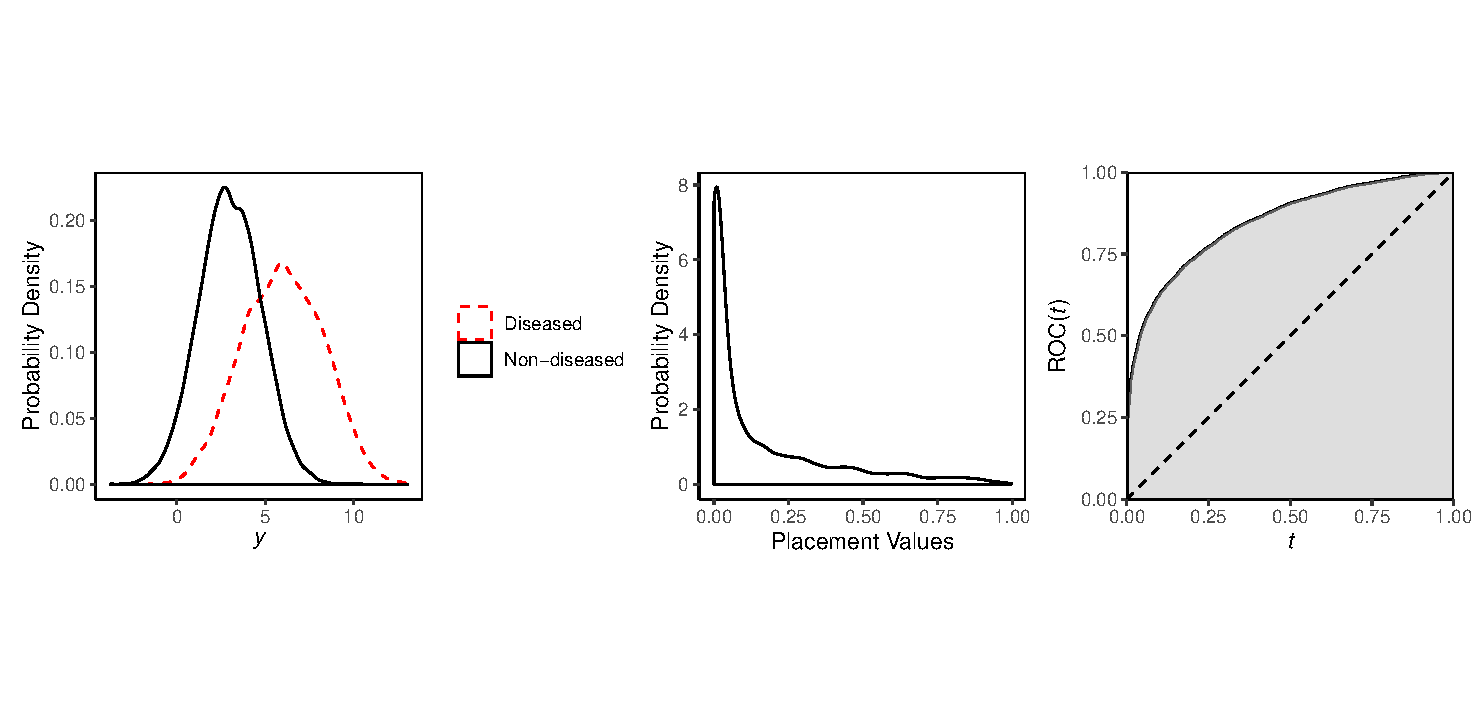
\includegraphics[width=4.5in]{PVs_ROC}
% \end{center}
% \end{frame}

%%%%% DIRECTION MODELING OF ROC CURVES
\section{Direct Modeling of ROC Curves}

\begin{frame}
\frametitle{BLAHH}
\begin{itemize}
\item Pepe (1997) introduced a general regression framework for modeling covariate effects on ROC curves. It has the form
\end{itemize}
$$\text{ROC}_{\matr{x}}(t) = g\left(h(t) + \matr{x}^{\prime}\bm{\beta}\right),$$
\vspace{-.2in}
\begin{itemize}
\item[] where $g(\cdot)$ is a monotone increasing function with range $(0, 1)$, $h(t) = \sum_{k=1}^K \gamma_kh_k(t)$ is an increasing function on the domain $(0 ,1)$ with associated unknown parameters $\gamma_k, \, k = 1, \dots, K,$ and $\matr{x}$ is a $p \times 1$ vector of covariates with associated unknown regression coefficients $\bm{\beta}$ $(p \times 1)$.
\item This approach is known as parametric distribution-free (PDF) because it specifies a parametric model for the ROC curve but does not make any distributional assumptions about $Y$.
%the test results.
\end{itemize}
\end{frame}


%%%%% PDF ROC USING BINARY REGRESSION TECHNIQUES
\section{PDF ROC Using Binary Regression Techniques}

\begin{frame}
\frametitle{BLAHH}
\begin{itemize}
\item Alonzo and Pepe (2002) proposed an estimation procedure based on binary indicators:
\end{itemize}
$$U_{it} = I[Y_{D_i} \geq S_{\bar{D}, \matr{x}_i}^{-1}(t)], \quad \text{for } t \in T \text{ and } i = 1, \dots, n_D,$$
\vspace{-.2in}
\begin{itemize}
\item[] where $t$ is a FPR and $T$ denotes a fixed finite set of FPRs.
\item The crucial result is 
\end{itemize}
\vspace{-.15in}
\begin{align*}
\text{E}[U_{it}] &= P(Y_{D_i} \geq S_{\bar{D},\matr{x}_i}^{-1}(t)) \\
&= S_{D,\matr{x}_i}(S_{\bar{D},\matr{x}_i}^{-1}(t)) \\
&= \text{ROC}_{\matr{x}_i}(t) \\
&= g\left(\sum_{k=1}^K\gamma_kh_k(t) + \matr{x}_i^{\prime}\bm{\beta}\right).
\end{align*}
\end{frame}

%%%%% PDF ALGORITHM
% \section{PDF Algorithm}

% \begin{frame}
% 	\frametitle{BLAHH}
% 	{\color{red} Don't Need}
% 	\begin{enumerate}
% 		\item Specify a set $T = \left\{j/n_T,\, j = 1, \dots, n_{T-1}, \, n_T \leq n_{\bar{D}}\right\}$ of FPRs to consider.
% 		\item For each $t \in T$, estimate $S_{\bar{D},\matr{x}_i}^{-1}(t)$.
% 		\item Calculate the binary indicator $U_{it} = I[Y_{D_i} \geq \hat{S}_{\bar{D},\matr{x}_i}^{-1}(t)]$ for $t \in T$ and $i = 1, \dots, n_D$.
% 		\item Fit the model $\text{E}[U_{it}] = g\left(\sum_{k=1}^K \gamma_kh_k(t) + \matr{x}_i^{\prime}\bm{\beta}\right)$.
% 	\end{enumerate}
% \end{frame}

%%%%% BETA ROC
\section{Beta ROC}

\begin{frame}
	\frametitle{BLAHH}
	\begin{itemize}
		\item Stanley and Tubbs (2018) introduced a Beta regression approach to estimate the covariate-specific ROC curve.
		\item This method utilizes Beta regression to directly model placement values.
		\begin{itemize}
		    \item The Beta regression model is related to the generalized linear model (GLM) framework.
		    \item The cdf of the fitted $\text{Beta}(a, b)$ model of placement values (given covariates) provides an estimate of the ROC curve.
		\end{itemize}
	\end{itemize}
\end{frame}

%%%%% BETA REGRESSION MODEL
\section{Beta Regression Model}

\begin{frame}
	\frametitle{BLAHH}
	\begin{itemize}
		\item For a dependent variable $Y$ distributed $\text{Beta}(a, b)$, the usual form of the beta density is 
	\end{itemize}
$$f(y; a, b) = \frac{\Gamma(a + b)}{\Gamma(a)\Gamma(b)}y^{a-1}(1 - y)^{b-1}, \quad 0 < y < 1,$$
\vspace{-.2in}
\begin{itemize}
	\item[] where $a, b > 0$ and $\Gamma(\cdot)$ is the gamma function.
\end{itemize}
$$\text{E}[Y] = \frac{a}{a+b} \quad \text{ and } \quad \text{Var}(Y) = \frac{ab}{(a + b)^2(a + b + 1)}.$$
\vspace{-.2in}
\begin{itemize}
	\item Ferrari and Cribari-Neto (2004) developed a beta regression model parameterized by mean and precision parameters, $\mu = \text{E}[Y]$ and $\phi = a + b$, respectively.
	$$\text{E}[Y] = \mu \quad \text{ and } \quad \text{Var}(Y) = \frac{\mu(1 - \mu)}{1 + \phi}.$$
\end{itemize}
\end{frame}

%%%%% MODELING PLACEMENT VALUES USING BETA REGRESSION
\section{Modeling Placement Values Using Beta Regression}

\begin{frame}
	\frametitle{BLAHH}
	\begin{itemize}
		\item The $\text{PV}_i, \, i = 1, \dots, n_{D},$ can be modeled as $\text{Beta}(\mu_i, \phi)$ random variables.
		\item The beta regression model is written as
	\end{itemize}
$$g(\mu_i) = \matr{x}_i^{\prime}\bm{\beta},$$
	\vspace{-.2in}
	\begin{itemize}
		\item[] where $\bm{\beta}$ is a $(k + 1) \times 1$ vector of unknown regression parameters, $\matr{x}_i = (1, x_{i1}, \dots, x_{ik})^{\prime}$ is a vector of observations on $k$ covariates, and $g(\cdot)$ is a monotone link function.
	\end{itemize}
\vspace{-.15in}
\begin{align*}
\text{E}[\text{PV}_i|\matr{x}_i] &= \mu_i = g^{-1}(\matr{x}_i^{\prime}\bm{\beta}) \\
\text{Var}(\text{PV}_i|\matr{x}_i) &=  \frac{\mu_i(1 - \mu_i)}{1 + \phi} = \frac{g^{-1}(\matr{x}_i^{\prime}\bm{\beta})\left[1 - g^{-1}(\matr{x}_i^{\prime}\bm{\beta})\right]}{1 + \phi}.
\end{align*}
\end{frame}

%%%%% MODELING PLACEMENT VALUES USING BETA REGRESSION
\section{Modeling Placement Values Using Beta Regression}

\begin{frame}
	\frametitle{BLAHH}
	\begin{itemize}
		\item When the logit link is used, it follows that
	\end{itemize}
$$\text{E}[\text{PV}_i|\matr{x}_i] = \mu_i = \frac{1}{1 + \exp\left\{-\matr{x}_i^{\prime}\bm{\beta} \right\}}.$$
\begin{itemize}
\item[] In which case,  %Consequently, we can obtain the usual $a$ and $b$ shape parameters for the beta distribution.
\end{itemize}
%\begin{minipage}{0.47\textwidth}
\vspace{-.15in}
\begin{eqnarray*}
a = \mu\phi 
	= \frac{\phi}{1 + \exp\left\{-\matr{x}_i^{\prime}\bm{\beta}\right\}}
\end{eqnarray*}
\vspace{-.2in}
%\end{minipage}
%\begin{minipage}{0.5\textwidth}
\begin{itemize}
\item[] and
\end{itemize}
\vspace{-.15in}
	\begin{eqnarray*}
	b = (1 - \mu)\phi 
		= \phi\left(1 - \frac{1}{1 + \exp\left\{-\matr{x}_i^{\prime}\bm{\beta}\right\}} \right)
	\end{eqnarray*}
%\end{minipage}
\end{frame}

%%%%% BETA ALGORITHM
% \section{Beta Algorithm}

% \begin{frame}
% 	\frametitle{BLAHH}
% 	{\color{red} Don't Need}
% 	\begin{enumerate}
% 		\item Specify a set $T = \left\{j/n_T,\, j = 1, \dots, n_{T-1}, \, n_T \leq n_{\bar{D}}\right\}$ of FPRs to consider.
% 		\item For each $t \in T$, estimate $S_{\bar{D},\matr{x}_i}^{-1}(t)$.
% 		\item Calculate the placement values, $\text{PV}_i = \hat{S}_{\bar{D},\matr{x}_i}(Y_{D_i})$.
% 		\item Fit a beta regression model to the placement values, thereby obtaining estimates of $\bm{\beta}$ and $\phi$.
% 		\item Acquire the shape parameters $a = \mu\phi$ and $b = (1 - \mu)\phi$.
% 		\item Calculate the cdf of the placement values with the $\text{Beta}(a, b)$ distribution in \textcolor{BaylorBrown}{5.} to estimate the ROC and AUC.
% 	\end{enumerate}
% \end{frame}
 
%%%%% VARIABLE DISPERSION BETA REGRESSION MODEL
\section{Variable Dispersion Beta Regression Model}

\begin{frame}
	\frametitle{BLAHH}
	\begin{itemize}
		\item Smithson and Verkuilen (2006) extended the beta regression model by proposing that the precision parameter can be modeled with its own set of covariates. 
		\item In their model, $Y_i \sim \text{Beta}(\mu_i, \phi_i), \, i = 1, \dots, n$, and 
	\end{itemize}
\vspace{-.1in}
\begin{align*}
g(\mu_i) &= \matr{x}_i^{\prime}\bm{\beta}, \\
h(\phi_i) &= \matr{w}_i^{\prime}\bm{\delta}, \\
\end{align*}
\vspace{-.4in}
\begin{itemize}
	\item[] where $\bm{\beta} = (\beta_0, \beta_1, \dots, \beta_k)^{\prime}$ and $\bm{\delta} = (\delta_0, \delta_1, \dots, \delta_l)^{\prime}$ are vectors of unknown regression parameters, $\matr{x}_i = (1, x_{i1}, \dots, x_{ik})^{\prime}$ and $\matr{w}_i = (1, w_{i1}, \dots, w_{il})^{\prime}$ are (potentially overlapping or identical) vectors of observations on $k$ and $l$ covariates, respectively, and $g(\cdot)$ and $h(\cdot)$ are monotone link functions. 
\end{itemize}
\end{frame}

%%%%% MODELING PLACEMENT VALUES WITH THE VARIABLE DISPERSION BETA REGRESSION MODEL
\section{Modeling Placement Values with the Variable Dispersion Beta Regression Model}

\begin{frame}
	\frametitle{BLAHH}
	\begin{itemize}
		\item The $\text{PV}_i, \, i = 1, \dots, n_{D},$ can be modeled as $\text{Beta}(\mu_i, \phi_i)$ random variables.
		\item Employing the logit link for $\mu_i$ gives
	\end{itemize}
$$\text{E}[\text{PV}_i|\matr{x}_i] = \mu_i = \frac{1}{1 + \exp\left\{-\matr{x}_i^{\prime}\bm{\beta}\right\}}.$$
\vspace{-.2in}
	\begin{itemize}
		\item Employing the log link for $\phi_i$ gives
	\end{itemize}
$$\phi_i = \exp\left\{\matr{w}_i^{\prime}\bm{\delta}\right\}.$$
\vspace{-.2in}
\begin{itemize}
	\item As in the Beta ROC algorithm, the shape parameters for the beta distribution can be obtained, and the ROC and AUC can be estimated as a result.
\end{itemize}
\end{frame}

%%%%% THE BINORMAL ROC CURVE
\section{The Binormal ROC Curve}

\begin{frame}
	\frametitle{BLAHH}
If 
$$Y_D \sim \text{N}(\mu_D, \sigma^2_D), \quad Y_{\bar{D}} \sim \text{N}(\mu_{\bar{D}}, \sigma^2_{\bar{D}}),$$

then
$$\text{ROC}(t) = \Phi(a + b\,\Phi^{-1}(t)), \quad t \in (0, 1),$$

and
$$\text{AUC} = \Phi\left(\frac{a}{\sqrt{1 + b^2}}\right),$$
	
where
$$a = \frac{\mu_D - \mu_{\bar{D}}}{\sigma_D}, \quad b = \frac{\sigma_{\bar{D}}}{\sigma_{D}}.$$
\end{frame}

%%%%% BINORMAL ROC SIMULATION
\section{Binormal ROC Simulation}

\begin{frame}
	\frametitle{BLAHH}
	\begin{itemize}
		\item We simulated 1,000 datasets from
	\end{itemize}
\begin{align*}
Y_D &= 2 + 4X + \varepsilon_D, \\
Y_{\bar{D}} &= 1.5 + 3X + \varepsilon_{\bar{D}}, \\
\end{align*}
\vspace{-.4in}
\begin{itemize}
	\item[] where $X \sim \text{Uniform}(0, 1)$ and $\varepsilon_{D}, \varepsilon_{\bar{D}} \sim \text{N}(0, 1.5^2)$.
	\item At $X = x_0$, the binormal ROC curve and AUC are respectively 
\end{itemize}
\begin{align*}
\text{ROC}(t) &= \Phi\left(\frac{1}{3} + \frac{2}{3}x_0 + \Phi^{-1}(t)\right), \quad t \in (0, 1), \\
\text{AUC} &= \Phi\left(\frac{0.5 + x_0}{\sqrt{4.5}}\right).
\end{align*}
\end{frame}

%%%%% BINORMAL ROC SIMULATION RESULTS
\section{Binormal ROC Simulation Results}

\begin{frame}
	\frametitle{BLAHH}
	\begin{itemize}
		\item We compared the  average of the 1,000 estimated ROC curves and corresponding AUCs at various covariate values for each of the three methods:
		\begin{enumerate}
			\item Parametric distribution-free (PDF)
			\item Beta
			\item Variable Dispersion Beta (VD Beta)
		\end{enumerate}
	\vspace{-.075in}
	\end{itemize}
	  \begin{center}
		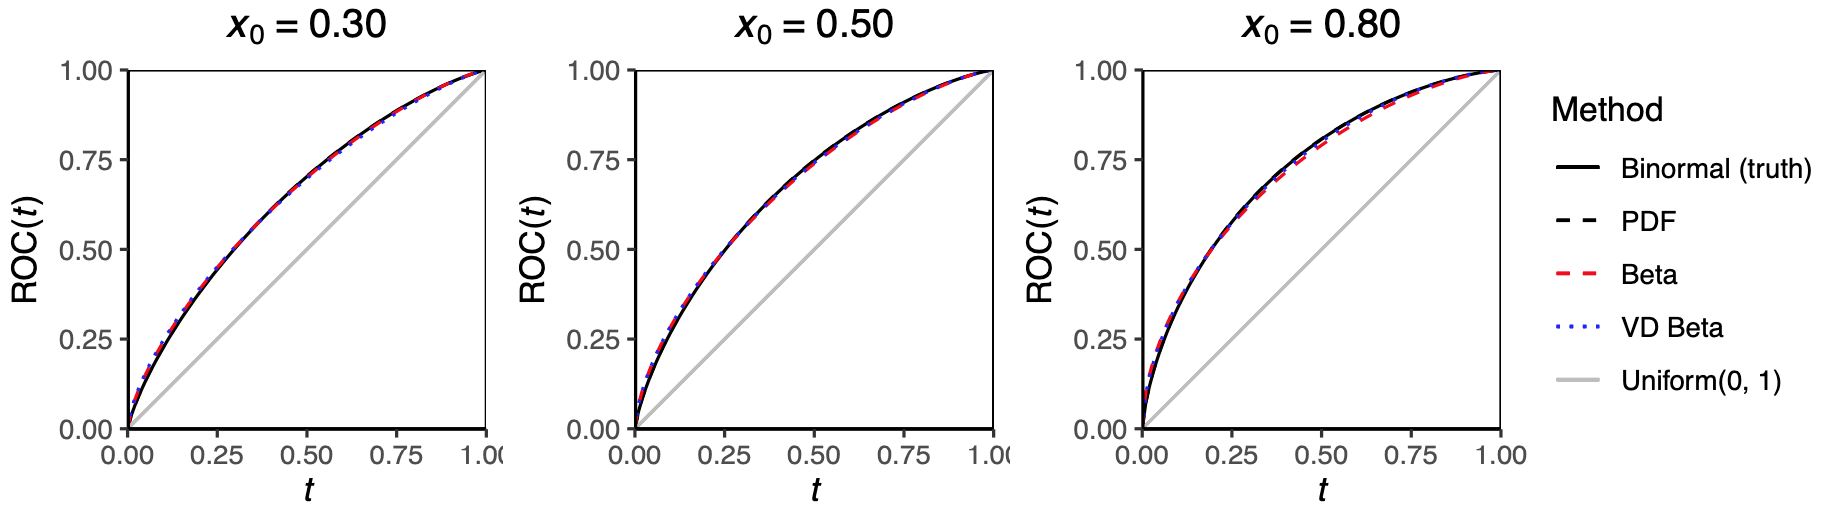
\includegraphics[scale=0.3]{sim_results}
	\end{center}
\vspace{-.1in}
		\begin{table}[ht]
	\centering
	\begin{threeparttable}
		\scalebox{0.5}{
		\begin{tabular}{l c c c c}
			% \vspace{-7mm} \\
			\hline
			& & \multicolumn{3}{c}{$x_0$} \\
			\cline{3-5} \\
			AUC & & 0.30 & 0.50 & 0.80 \\
			\hline
			\addlinespace[1ex] Binormal (truth) & & 0.647 & 0.681 & 0.730 \\
			\addlinespace[1ex] PDF & & 0.647 & 0.682 & 0.730 \\
			\addlinespace[1ex] \textcolor{red}{Beta} & & 0.649 & 0.680 & 0.724 \\
			\addlinespace[1ex] \textcolor{blue}{VD Beta} & & 0.648 & 0.682 & 0.729 \\
			\hline
		\end{tabular}}
	\end{threeparttable}
		\end{table}
\end{frame}

%%%%% APPLICATION TO INDIAN LIVER PATIENT DATASET
\section{Application to Indian Liver Patient Dataset}

\begin{frame}
	\frametitle{BLAHH}
	\begin{itemize}
		\item Evaluate total bilirubin as a predictive marker for liver disease.
		\item Higher levels of total bilirubin can be an indicator of improper liver functioning.
		\item Of the 545 subjects age $\geq 20$, 133 ($24.4\%$) are female and 412 ($76.6\%$) are male. Also, $394 / 545 = 72.3\%$ of subjects are liver patients.
		\item Questions of interest:
		\begin{itemize}
			\item How well does total bilirubin distinguish between liver patients and healthy patients?
			\item Do covariates gender and albumin affect the discrimination ability of total bilirubin?
		\end{itemize}
	\end{itemize}
\end{frame}

%%%%% APPLICATION TO INDIAN LIVER PATIENT DATASET
\section{Application to Indian Liver Patient Dataset}

\begin{frame}
	\frametitle{BLAHH}
	\begin{itemize}
		\item The empirical ROC curve for total bilirubin discriminates fairly well ($\text{AUC} = 0.693$).
	\end{itemize}
\begin{center}
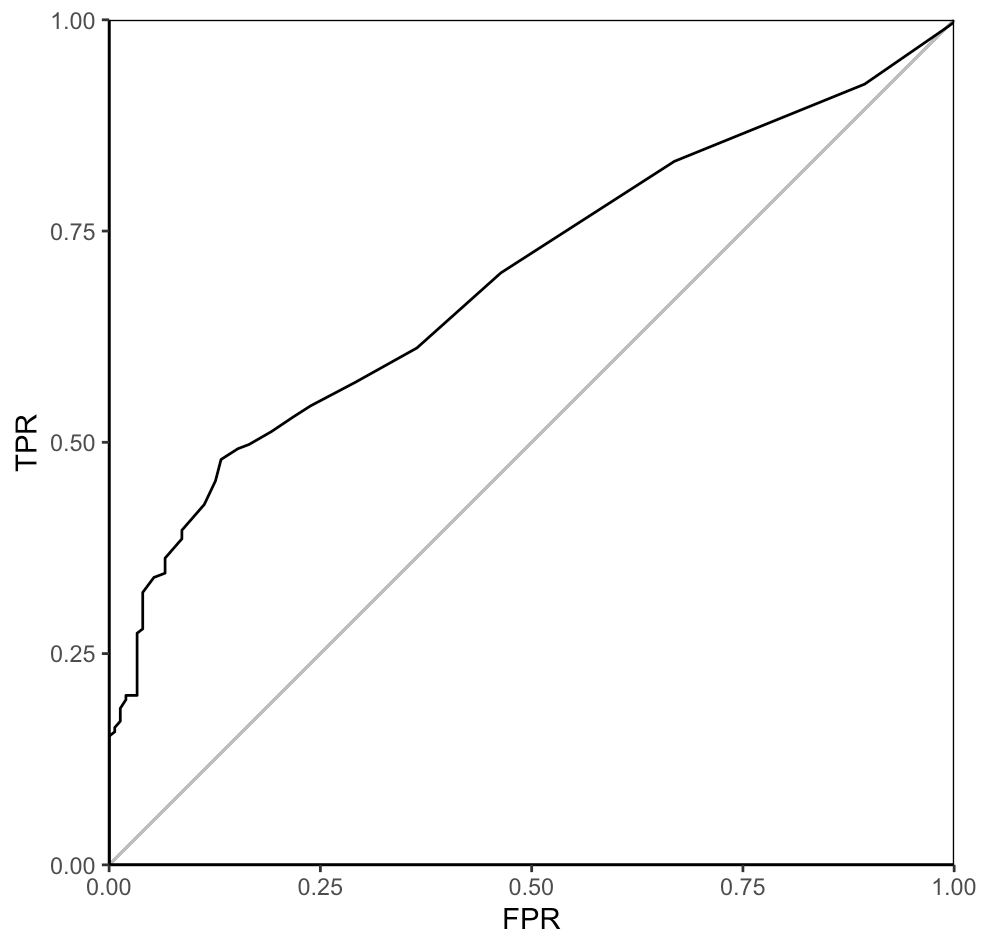
\includegraphics[width = 2.5in]{ilpd_emp}
\end{center}
\end{frame}

%%%%% RESULTS OF BETA ROC REGRESSION ON THE INDIAN LIVER PATIENT DATASET
\section{Results of Beta ROC Regression on the Indian Liver Patient Dataset}

\begin{frame}
	\frametitle{BLAHH}
	\begin{center}
	\begin{threeparttable}
		\scalebox{0.75}{
			\begin{tabular}{l c c c c}
				% \vspace{-7mm} \\
				\hline
				\addlinespace[1ex]  \textbf{Coefficients (mean model with logit link)}  & & Estimate & Standard error & $p$-value \\
				\hline
				\addlinespace[1ex] $\beta_0$ & & $-1.470$ & 0.289 & $< 0.001$ \\
				\addlinespace[1ex] $\beta_1$ (Gender: female $=0$, male $=1$) & & $-0.191$ & 0.151 & 0.204 \\
				\addlinespace[1ex] $\beta_2$ (Albumin) & & 0.299 & 0.079 & $< 0.001$ \\
				\hline
				\addlinespace[1ex] \textbf{Precision} & & Estimate & Standard error & $p$-value  \\
				\hline
				\addlinespace[1ex] $\phi$ & & $1.135$ & 0.069 & $< 0.001$ \\
				\hline
		\end{tabular}}
	\end{threeparttable}
\end{center}
\begin{small}
	\begin{itemize}
		\item The estimated coefficients for the mean model can be interpreted in terms similar to odds ratios or more generally as conditional means of the placement values.
		\item The negative coefficient for \texttt{Gender} means that the average placement value is smaller for males than females $\Rightarrow$ better separation in males.
		\item The positive coefficient for \texttt{Albumin} means that the average placement value is larger for higher albumin levels $\Rightarrow$ better separation for lower albumin levels.
	\end{itemize}
\end{small}
\end{frame}


%%%%% RESULTS OF VARIABLE DISPERSION BETA ROC REGRESSION ON THE INDIAN LIVER PATIENT DATASET
\section{Results of Variable Dispersion Beta ROC Regression on the Indian Liver Patient Dataset}

\begin{frame}
	\frametitle{BLAHH}
		
	\begin{center}
		\begin{threeparttable}
			\scalebox{0.75}{
				\begin{tabular}{l c c c c}
					% \vspace{-7mm} \\
					\hline
					\addlinespace[1ex] \textbf{Coefficients (mean model with logit link)}& & Estimate & Standard error & $p$-value \\
					\hline
					\addlinespace[1ex] $\beta_0$ & & $-1.780$ & 0.309 & $< 0.001$ \\
					\addlinespace[1ex] $\beta_1$ (Gender: female $=0$, male $=1$) & & $-0.122$ & 0.157 & 0.437 \\
					\addlinespace[1ex] $\beta_3$ (Albumin) & & 0.374 & 0.085 & $< 0.001$ \\
					\hline
					\addlinespace[1ex] \textbf{Phi coefficients (precision model with log link)} & & Estimate & Standard error & $p$-value \\
					\hline
					\addlinespace[1ex] $\delta_0$ & & $0.889$ & 0.289 & $0.002$ \\
					\addlinespace[1ex] $\delta_1$ (Gender: female $=0$, male $=1$) & & $-0.214$ & 0.146 & 0.143 \\
					\addlinespace[1ex] $\delta_2$ (Albumin) & & $-0.187$ & 0.078 & $0.017$ \\
					\hline
			\end{tabular}}
		\end{threeparttable}
	\end{center}
	\begin{itemize}
		\item The negative coefficients for $\delta_1$ and $\delta_2$ indicate that higher values of those variables are associated with increased variability in the placement values.
	\end{itemize}
\end{frame}

%%%%% COMPARING ESTIMATES OF ROC AND AUC FOR THE INDIAN LIVER PATIENT DATASET
\section{Comparing Estimates of ROC and AUC for the Indian Liver Patient Dataset}

\begin{frame}
	\frametitle{BLAHH}
	\begin{center}
		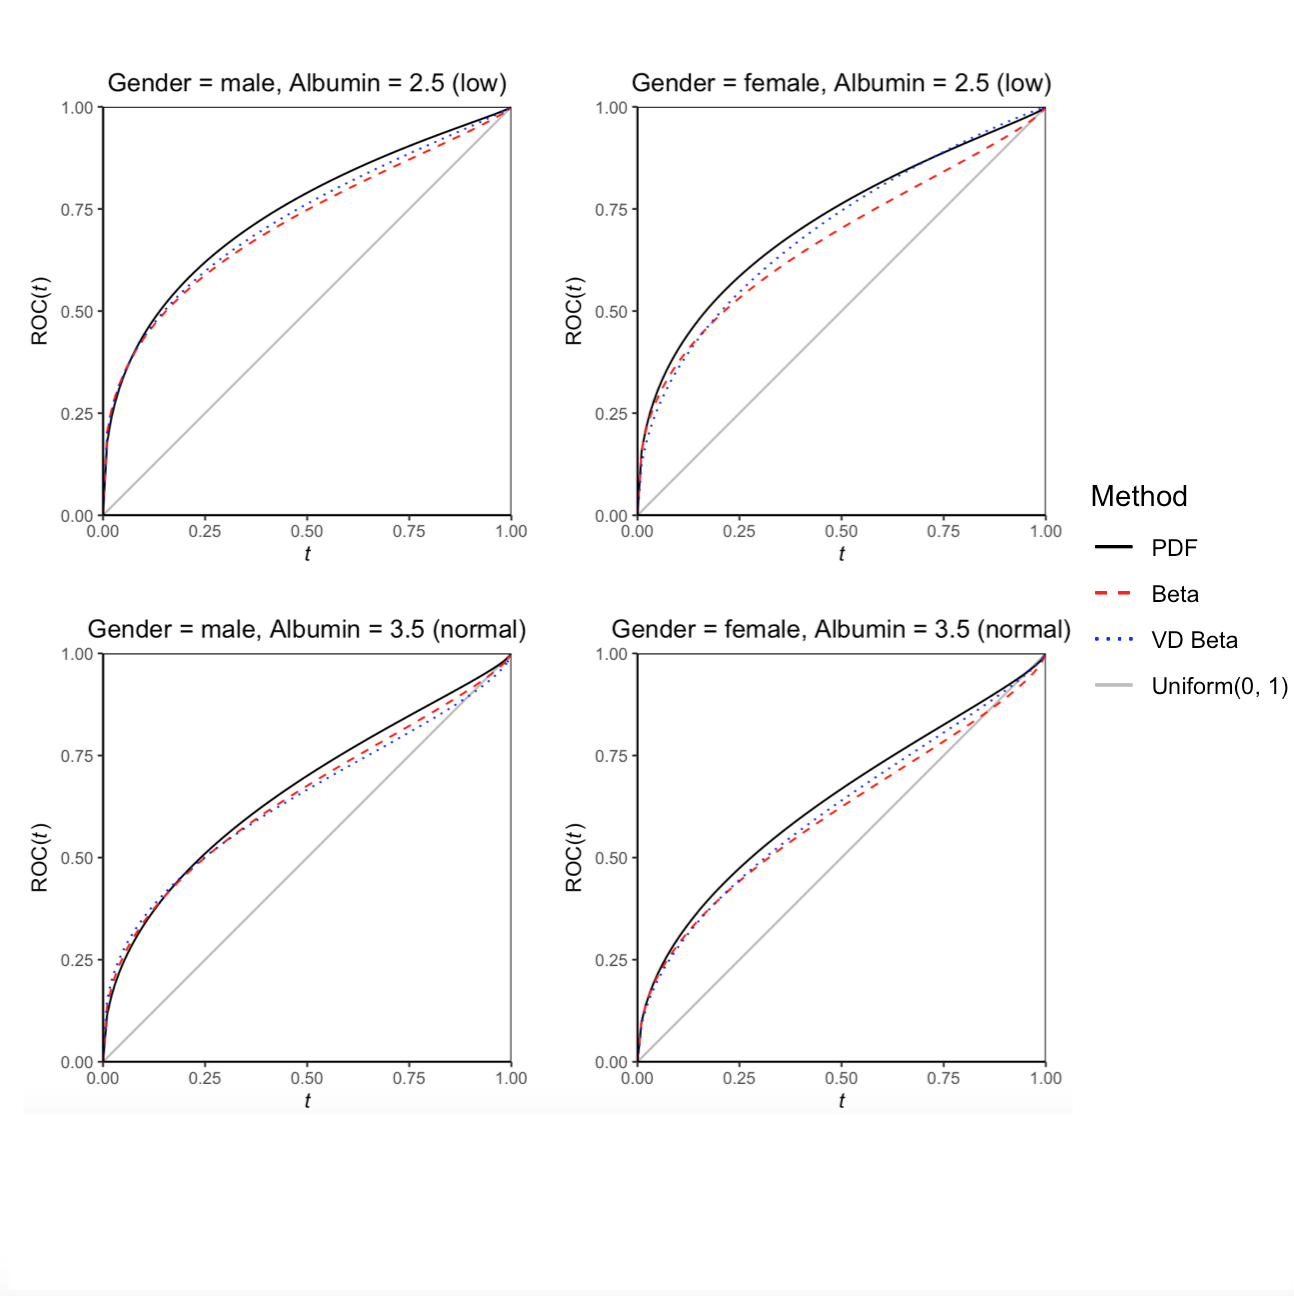
\includegraphics[scale=0.36]{tryin2}
	\end{center}
\end{frame}

\begin{frame}
	\frametitle{BLAHH}
\begin{center}
	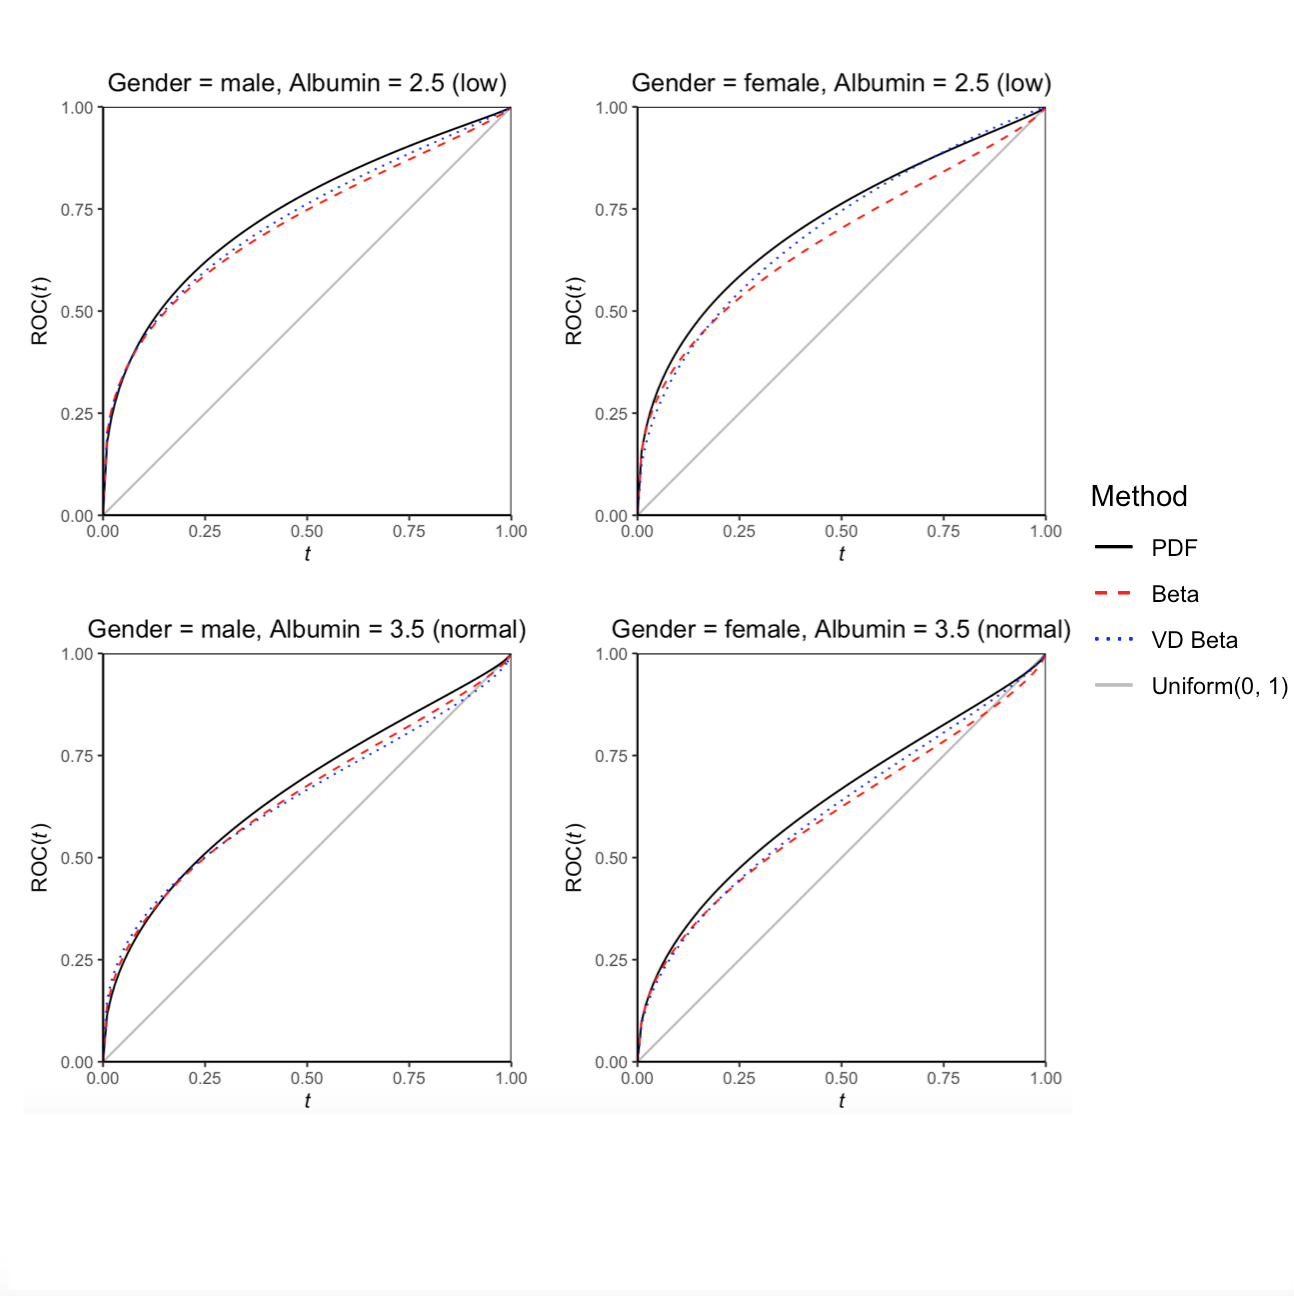
\includegraphics[scale=0.2]{tryin2}
\begin{threeparttable}
	\scalebox{0.5}{
		\begin{tabular}{l c c c c c}
			% \vspace{-7mm} \\
			\hline
			& & \multicolumn{4}{c}{Covariate settings} \\
			\cline{3-6} \\
			AUC & & Male, & Female, & Male, & Female, \\
			        & & Albumin $= 2.5$ & Albumin $= 2.5$ & Albumin $=3.5$ & Albumin $=3.5$ \\
			\hline
			\addlinespace[1ex] PDF & & 0.741 & 0.717 & 0.663 & 0.637  \\
			\addlinespace[1ex] \textcolor{red}{Beta} & & 0.714 & 0.673 & 0.649 & 0.605 \\
			\addlinespace[1ex] \textcolor{blue}{VD Beta} & & 0.724 & 0.699 & 0.644 & 0.615 \\
			\hline
	\end{tabular}}
\end{threeparttable}
\end{center}
\end{frame}

%%%%% CHOOSING BETWEEN MODELS
\section{Choosing Between Models}

\begin{frame}
	\frametitle{BLAHH}
	\begin{itemize}
		\item Likelihood ratio tests, AIC and BIC.
		\item Test different link functions for the mean parameter.
		\item Model fit diagnostics.
	\end{itemize}
\end{frame}


%%%%% CONCLUSION AND FUTURE WORK
\section{Conclusion and Future Work}

\begin{frame}
	\frametitle{BLAHH}
	\begin{itemize}
		\item Modeling placement values with a variable dispersion beta regression model yields estimated ROC curves and AUCs comparable to other methods.
		\item The variable dispersion beta regression model allows one to examine the variation of the placement values for various covariate settings.
		\item Talk about why you might want to use the Variable Dispersion Beta Regression Model to model the placement values.
		\item Future work: mixture of two betas..
	\end{itemize}
\end{frame}

%%%%% RFERENCES
\section{References}

\begin{frame}
	\frametitle{BLAHH}
	\begin{footnotesize}
	\begin{itemize}
		\item Alonzo, T. A., and Pepe, M. S. (2002), ``Distribution-free ROC analysis using binary regression techniques,’’ \textit{Biostatistics}, 3, 421–432.
		\item Ferrari, S., and Cribari-Neto, F. (2004), ``Beta Regression for Modelling Rates and Proportions,’’ \textit{Journal of Applied Statistics}, 31, 799–815.
		\item Hanley, J. A., and Mcneil, B. J. (1982), ``The meaning and use of the area under a receiver operating characteristic (ROC) curve,’’ \textit{Radiology}, 143, 29–36.
		\item Pepe, M. (1997), ``A regression modelling framework for receiver operating characteristic curves in medical diagnostic testing,’’ \textit{Biometrika}, 84, 595–608.
		\item Pepe, M. S., and Cai, T. (2004), ``The Analysis of Placement Values for Evaluating Discriminatory Measures,’’ \textit{Biometrics}, 60, 528–535. 
		\item Ramana, B. V., Babu, M. S. P., and Venkateswarlu, N. B. (2011),  ``A Critical Study of Selected Classification Algorithms for Liver Disease Diagnosis,’’ \textit{International Journal of Database Management Systems}, 3, 101–114.
		\item Smithson, M., and Verkuilen, J. (2006), ``A better lemon squeezer? Maximum-likelihood regression with beta-distributed dependent variables,’’ \textit{Psychological Methods}, 11, 54–71.
		\item Stanley, S., and Tubbs, J. (2018), ``Beta Regression for Modeling a Covariate Adjusted ROC,’’ \textit{Science Journal of Applied Mathematics and Statistics}, 6, 110–118.
	\end{itemize}
	\end{footnotesize}
\end{frame}



\end{document}